\documentclass[12pt]{article}
%\usepackage{caption} % improved spacing between figure and caption
\usepackage[utf8]{inputenc}
 \usepackage{bm}
\usepackage{amsmath}
 \usepackage{booktabs} 
 %\usepackage{pgfplots} 
% \usepackage{pgfplotstable} 
 \usepackage{multirow}
\newcommand{\Real}{\mathbb{R}}
 \newcommand{\dom}{{\bf dom}\,}
 \newcommand{\Tra}{^{\sf T}} % Transpose
 \newcommand{\Inv}{^{-1}} % Inverse
 \def\vec{\mathop{\rm vec}\nolimits}
 \def\sweep{\mathop{\rm sweep}\nolimits}
 \newcommand{\diag}{\mathop{\rm diag}\nolimits}
 \newcommand{\tr}{\operatorname{tr}} % Trace
 \newcommand{\epi}{\operatorname{epi}} % epigraph
 \newcommand{\V}[1]{{\bm{\mathbf{\MakeUppercase{#1}}}}} % vector
 \newcommand{\VE}[2]{\MakeLowercase{#1}_{#2}} % vector element
 \newcommand{\Vn}[2]{\V{#1}^{(#2)}} % n-th vector
 \newcommand{\Vtilde}[1]{{\bm{\tilde \mathbf{\MakeLowercase{#1}}}}} % vector
 \newcommand{\Vhat}[1]{{\bm{\hat \mathbf{\MakeLowercase{#1}}}}} % vector
 \newcommand{\VtildeE}[2]{\tilde{\MakeLowercase{#1}}_{#2}} % vector element
 \newcommand{\M}[1]{{\bm{\mathbf{\MakeUppercase{#1}}}}} % matrix
 \newcommand{\ME}[2]{\MakeLowercase{#1}_{#2}} % matrix element
 \newcommand{\Mtilde}[1]{{\bm{\tilde \mathbf{\MakeUppercase{#1}}}}} % matrix
 \newcommand{\Mhat}[1]{{\bm{\hat \mathbf{\MakeUppercase{#1}}}}} % matrix
 \newcommand{\Mcheck}[1]{{\bm{\check \mathbf{\MakeUppercase{#1}}}}} % matrix
 \newcommand{\Mbar}[1]{{\bm{\bar \mathbf{\MakeUppercase{#1}}}}} % matrix
 \newcommand{\Mn}[2]{\M{#1}^{(#2)}} % n-th matrix
 %artcle or book or beamer, letter 
%if use beamer, use \begin{frame}\end{frame}to begin a new slide, and do not use package{geometry}
\usepackage{fixltx2e}
\usepackage{graphicx}
\usepackage{longtable}
\usepackage{float}
\usepackage{wrapfig}
\usepackage{rotating}
\usepackage{hyperref}
%\usepackage[normalem]{ulem}
\usepackage{amsmath}
\usepackage{textcomp}
\usepackage{marvosym}
%\usepackage{wasysym}
\usepackage{amssymb}
\usepackage{multirow}
\usepackage{subfigure}
%\usepackage{listings}
%\usepackage[top=2cm,bottom=2cm]{geometry}%l\usepackage{latexsym}
\usepackage{listings}\lstset{breaklines}
%\usepackage[top=2cm,bottom=2cm]{geometry}
%\usepackage{extarrows}
%\usepackage{makecell}
\usepackage{array}
%\usepackage{natbib}
%\usepackage{cite}
%\usepackage{biblatex}
%\addbibresource{reference.bib}
 \usepackage{color}

 
 \def\E{\mathbb{E}}
 \def\R{\mathbb{R}}
 \def\T{\mathcal{T}}
 \def\ba{\mathbf{a}}
 \def\N{\mathcal{N}}
 \def\C{\mathcal{C}}
 
 \def\luo#1{{\bf \color{red} Luo: \color{blue} #1}}
 
\title{A functional mixed effect model for scalar on function regression with application to a fMRI pain study}
\author{Wanying Ma, Bowen Liu, Luo Xiao, Martin A.Lindquist}
\date{\today}
 
\begin{document}
\maketitle
\section{Introduction}
Recently, there has been a rapid emerge in the area of brain imaging study\cite{lindquist2008statistical, wager2008prefrontal,zipunnikov2011multilevel,huang2017two}. Scientific interest has raised in the potential relationship between the continuously observed brain activity trajectories with one's subjective reaction to certain experiment conditions\cite{lindquist2012functional}, results of the subject-level difference in the observed trajectories in the reaction, and thus how the brain activity interacts the psychological/physiological process. Equipped with instruments such as fMRI or EEG machine\cite{wang2016functional}, a functional brain activity curve can be noninvasively observed on the equally spaced time grid $t_1,\dots,t_p$ over time, that is, $t_{i+1}-t_{i}=t_{j+1}-t_j$, $\forall 1\le i,j\le p$. Functional magnetic resonance imaging, or functional MRI(fMRI) measures the brain activity noninvasively by detecting the change in the blood flow associated with the neuron. During the entire course of fMRI, a sequence of magnetic resonance imaging(MRI) are performed, with a number of volume elements, or voxels, placed evenly over the brain\cite{lindquist2008statistical}. At the mean time, subjects can be asked for a set of tasks in the brain imaging experiment. Therefore, fMRI provides people with both spatial and temporal resolution for brain mapping function in response for the experimental task, and facilitate people with a non-surgery technique for the neuron activity research purpose\cite{cohen2017computational}. Researchers have gained lots of insights in the connections between brain activity function and psychological/physiological reaction through modeling fMRI data. In this work, we mainly focus on exploring the effects of subject-level brain activity function on self-reporting response in the frame work of functional data analysis.

Functional data analysis plays an important role in dealing with densely observed data in the observational studies and clinical trials in the past decades\cite{goldsmith2015generalized,di2009multilevel,ramsay2006functional,ramsay2007applied,xiao2018fast,xiao2016fast, yao2005functional, mclean2015restricted, huang2014joint, xiao2014quantifying}. Monitored by the development of technology, one can observe full trajectories with repeated measurements during a time interval or at several discrete time points\cite{crainiceanu2009generalized, xiao2014quantifying, goldsmith2015generalized,xiao2016movement}. The methods and techniques in the development of functional data analysis have been extensitively overviewed \cite{ramsay2005functional, ramsay2007applied, wang2016functional}. Functional principal component analysis (FPCA) as a main tool in functional data analysis for dimension reduction and identifying the main directions in the covariance function has a long history\cite{ramsay1991some,kneip1994nonparametric, staniswalis1998nonparametric, yao2005functional, di2009multilevel,zipunnikov2011multilevel};




There has been a vast amount of applications using functional data analysis. Functional linear regressionFew methods has been developed to make good use of fully observed fMRI trajectory in stead of summarized statistics in the past decades\cite{cohen2017computational, lindquist2012functional}. These immense data reduction leads to an obscure picture on the brain activity change over time, and thus leaves the connection between subject's experimental response not well explained. The development of functional data analysis  Functional data analysis has great application in the area of physical activity dataMartin\cite{lindquist2012functional} incorporated the functional data analysis settings into the standard mediation model(SME), established a linear functional standard mediation model(lfSME), being able to identifiably explain the causal effects from the parameters in lfSME under certain conditions.

The remainder of this paper is organized as follows. Section 2 will explain the experiment for aggregating the data, explicitly describe steps on developing the functional linear mixed model and test procedures. Corresponding simulation study under different cases will be given in Section 3. The proposed methodology to a real data application on fMRI dataset will be given in Section 4. 

%%%%%%%%%%%%%%%%%%%%%%%
%%%%%%%%%%%%%%%%%%%%%%%
\section{Data and Method}
%%%%%%%%%%%%%%%%%%%%%%%
%%%%%%%%%%%%%%%%%%%%%%%
\subsection{Data from a fMRI pain study}
The following description of the fMRI data is mostly based on Martin's recent JASA paper \cite{lindquist2012functional} on the functional data analysis. In that experiment, a heat stimuli was applied at one of two different levels (high and low) to each of 20 subjects at each repetition for 18 seconds. In 14 seconds later than the stimulus each subject was asked to report the subjective pain rating and responded in a few seconds. During the entire course of the experiment, each subject's brain activity was measured by fMRI method. Therefore, functional MRI data was sampled from 21 diverse classic pain-responsive brain regions. Each sample regiment had 23 equidistant temporal measurements made every 2 seconds, totally covering a 46-second brain activity from the application of the heat stimuli to the subjective pain report. The same experiment was conducted on each subject multiple times but the number of the repetitions is unbalanced design ranging from 39 to 48.


Based on the description above, the matrix $M_{I\times J}$ denotes the design matrix of Brain activation data sampled at a particular voxel on 20 interviewees with 39-48 replication each during 46-second fMRI experiment in 23 sampling time points.

$$
M_{I\times J} = 
\begin{pmatrix}
M_{1,1}(t_1) & M_{1,1}(t_2) & \cdots & M_{1,1}(t_{23}) \\
M_{1,2}(t_1) & M_{1,2}(t_2) & \cdots & M_{1,2}(t_{23}) \\
\vdots  & \vdots  & \ddots & \vdots  \\
M_{n,J_n}(t_1) & M_{n,J_n}(t_2) & \cdots & M_{n,J_n}(t_{23})
\end{pmatrix}
$$



Without the consideration on the subjective random error in the population, denote $y_{ij}$ as the subjective rating at $i$th subject in $j$th replication, $Z_{ij}$ as the indicator variable of thermal stimuli level at $i$th subject in $j$th replication whose value 1 for the high level and 0 for the low level, $\delta$ and $\gamma$ as the parameters of the general linear model, $M_{ij}(t)$ as the temporal functional covariate of the brain activation at a particular voxel in fMRI data set, $\beta(t)$ as the corresponding functional curve and $\epsilon_{ij}$ as the white error. The mean mixed model is described as $y_{ij} = \delta + \gamma Z_{ij} + \int \beta(t) M_{ij}(t) \, \mathrm{d}t + \epsilon_{ij}$, where $\epsilon_{ij}$ is i.i.d. across $i$ and $j$ and $\epsilon_{ij} \sim N(0, \sigma^2)$.  

However, based on our previous knowledge on that fMRI data across experimental interviewees, the individual random effect accounts for the causal effect on the thermal pain rating across different subjects. In order to explain the subjective error drawn from the population we consider, the individual-level random error terms are affiliated to each fixed parameter and parameter curve. 
Therefore, the extended functional mixed effect model is formed as the following.


The underlying distribution on $y_{ij}$ based on the model we formulate is of our interest, but the integration on the temporal random effect curve is the obstacle in the routine of functional regression analysis. On approach in fitting the functional mixed model is to assemble the sampling distribution and the conditional distribution $y_{ij}|\beta_i$ which maintains a simple form and relatively easy to be estimated.  

Based on the assumption above on $E(\beta_i) = 0$ and $COV[\beta_i(s), \beta_i(t)] = K(s, t)$, the complex structure of the functional covariance results in great computational burden in maximum likelihood method and large bias in method of moment. In order to simplify the model, the assumption on the functional covariance should be made.


\luo{I started working from here}.
%%%%%%%%%%%%%%%%%%%%%%%%%%%
%%%%%%%%%%%%%%%%%%%%%%%%%%%
%%%%%%%%%%%%%%%%%%%%%%%%%%%
\section{Functional mixed effects model for scalar on function regression with repeated outcomes}
%%%%%%%%%%%%%%%%%%%%%%%%%%%
%%%%%%%%%%%%%%%%%%%%%%%%%%%
%%%%%%%%%%%%%%%%%%%%%%%%%%%
To model subject-specific random effect of a functional predictor,
 we propose a novel functional mixed effect model extending
 the scalar on function linear regression for repeated outcomes. 
 The proposed model is
\begin{equation}
\label{eq:model}
Y_{ij} = \alpha + Z_{ij} (\gamma + \gamma_i)  + \int \left \{\beta(t) + \beta_i(t)\right\} X_{ij}(t) \, \mathrm{d}t + \epsilon_{ij},
\end{equation}
where $\alpha$ is the population intercept, $\gamma$ is the population effect of $Z_{ij}$, 
$\gamma_i$ is the random subject-specific effect of $Z_{ij}$ for subject $i$,
$\beta(\cdot)$ is the population effect of the functional predictor $M_{ij}(t)$, 
$\beta_i(\cdot)$ is the random subject-specific effect of the functional predictor,
and $\epsilon_{ij}$s are independently  and identically distributed (i.i.d.) random errors with distribution $\N(0,\sigma_{\epsilon}^2)$.
We assume that $\gamma_i$s are i.i.d. with distribution $\N(0,\sigma^2_\gamma)$, $\beta_i(\cdot)$s are i.i.d. random functions following a Gaussian process over $\T$ with mean function $\E\{\beta_i(t)\} = 0$ and covariance function $\text{cov}\{\beta_i(s),\beta_i(t)\} = \C(s,t)$, and all random terms are independent across subjects and from each other. 

%%%%%%%%%%%%%%%%%%%%%%%%%%%
%%%%%%%%%%%%%%%%%%%%%%%%%%%
%%%%%%%%%%%%%%%%%%%%%%%%%%%
\subsection{Model estimation}
%%%%%%%%%%%%%%%%%%%%%%%%%%%
%%%%%%%%%%%%%%%%%%%%%%%%%%%
The key idea is  to reduce model \eqref{eq:model}
to a linear mixed effects model using the functional principal component 
analysis (fPCA) of the functional predictor.
Specifically,  assume that $X_{ij}(\cdot)$ are independent random functions from a Gaussian process
with a mean function $\E\{X_{ij}(t)\}=\mu(t)$ and covariance function
$\text{cov}\{X_{ij}(s), X_{ij}(t)\}= \mathcal{K}(s,t)$.
The observed functional predictor might be contaminated with measurement errors. Thus, we consider
the model for the functional predictor
\begin{equation}
\label{eq:W}
W_{ijk} = X_{ij}(t_k) + e_{ijk},
\end{equation}
where $W_{ijk}$ is the observation at time $t_k$ for subject $i$ during visit $j$ and
$e_{ijk}$s are measurement errors that are independent across $i$, $j$ and $k$ and
are independent from the true random functions $X_{ij}(\cdot)$s.
Note that model \eqref{eq:W} has a two-level nested structure, and
a more complicated fPCA method such as the multilevel fPCA \cite{di2009multilevel}
may be employed. For simplicity, we assume that $X_{ij}(\cdot)$ are independent across subjects and visits.
By Meyer's theorem, $\mathcal{K}(s,t)$ can be decomposed as $\sum_{k=1}^{\infty} \lambda_k \phi_k(s)\phi_k(t)$,
where $\lambda_1\geq\lambda_2\geq\cdots \geq 0$ are non-increasing eigenvalues with associated
eigenfunctions $\phi_k(\cdot)$s that satisfy $\int_{\T} \phi_k(s)\phi_\ell(s) ds = 1_{\{k=\ell\}}$.
Here $1_{\{\cdot\}}$ is 1 if the statement inside the bracket is true and 0 otherwise.
Then by the Karhunen-Loeve expansion, $X_{ij}(\cdot)$ can be written as a linear combination of the eigenfunctions,
i.e., $X_{ij}(t) = \mu(t) + \sum_{k=1}^{\infty}\xi_{ijk} \phi_k(t)$, where $\xi_{ijk}$s are independent
 random scores with $\xi_{ijk}\sim \N(0,\lambda_k)$.
The fPCA can be conducted using the fast covariance estimation (FACE) method  \cite{xiao2016fast},
which is based on penalized splines and is implemented in the R function ``fpca.face" in the R package {\it refund}.
Then, we obtain estimates of the eigenfunctions, $\hat{\phi}_k(\cdot)$, and estimates of the eigenvalues, $\hat{\lambda}_k$.
The random scores $\xi_{ijk}$ can also be predicted, denoted by $\hat{\xi}_{ijk}$; see \cite{xiao2016fast} for more details.

For model identifiability, we assume that $\beta(\cdot)$ can also be written as a linear combination of the eigenfunctions
so that $\beta(t) = \sum_{k=1}^{\infty} \theta_k \phi_k(t)$, where $\theta_k$s are associated scalar coefficients to be determined.
Similarly, let $\beta_i(\cdot) = \sum_{k=1}^{\infty} \theta_{ik}\phi_k(t)$, where $\theta_{ik}$s are independent subject-specific
random coefficients with distribution $\N(0,\tau_k^2)$, where $\tau_k^2\geq 0$ are to be determined as well.
Note that the induced covariance function $\C(s,t)$ equals $\sum_{k\geq 1} \tau_k^2 \phi_k(s)\phi_k(t)$.
It follows that model \eqref{eq:model} can be rewritten as

\begin{equation}
\label{eq:lme}
Y_{ij} = \alpha + Z_{ij}(\gamma + \gamma_i)  + \sum_{k=1}^{\infty} \xi_{ijk} (\theta_{k} + \theta_{ik}) + \epsilon_{ij}.
\end{equation}

Model \eqref{eq:lme} has infinitely many parameters and hence can be not be fitted, a well known problem for scalar on
function regression. We follow the standard approach by truncating the number of eigenfunctions for approximating
the functional predictor, so that the associated scores and parameters for $\beta(\cdot)$ and $\beta_i(\cdot)$ are all finite dimensional.
Specifically, %denote the estimated eigenfunctions by $\hat{\phi}_k(\cdot)$ and the predicted scores by $\hat{\xi}_{ijk}$.
let $K$ be the number of eigenfunctions to be selected.
 Then an approximate and identifiable model is
\begin{equation}
\label{eq:lme:approx}
Y_{ij} = \alpha + Z_{ij}(\gamma + \gamma_i)  + \sum_{k=1}^{K} {\xi}_{ijk} (\theta_{k} + \theta_{ik}) + \epsilon_{ij}.
\end{equation}
Model \eqref{eq:lme:approx} is a linear mixed effects model and can be easily fitted by standard software.

In practice, the number of eigenfunctions $K$ is selected by AIC \cite{yao2005functional}.
Denote the selected number by $\hat{K}$. Then a practical model for \eqref{eq:lme:approx}
is
\begin{equation}
\label{eq:lme:prac}
Y_{ij} = \alpha + Z_{ij}(\gamma + \gamma_i)  + \sum_{k=1}^{\hat{K}} \hat{\xi}_{ijk} (\theta_{k} + \theta_{ik}) + \epsilon_{ij}.
\end{equation}
Denote the corresponding estimates of $\theta_k$ by $\hat{\theta}_k$ and the prediction of $\theta_{ik}$ by $\hat{\theta}_{ik}$.
Then,  $\hat{\beta}(t) = \sum_{k=1}^{\hat{K}} \hat{\theta}_k\hat{\phi}_k(t)$
and $\hat{\beta}_i(t) = \sum_{k=1}^{\hat{K}} \hat{\theta}_{ik}\hat{\phi}_k(t)$.

%%%%%%%%%%%%%%%%%%%%%%%%%%%
%%%%%%%%%%%%%%%%%%%%%%%%%%%
\section{Test of random functional effect}
%%%%%%%%%%%%%%%%%%%%%%%%%%%
%%%%%%%%%%%%%%%%%%%%%%%%%%%
The interest is to assess if the functional
effect is subject specific or the same across subjects.
In other words, if $\beta_i(t) =0$ for all $i$ and $t\in \T$ in model \eqref{eq:model}
or $\beta_i(t)\neq 0$ for some $i$ at some $t\in \T$. 
Because $\beta_i(\cdot)$s are random coefficient functions,
the test can be formulated in terms of its covariance function.
The null hypothesis is $H_0: \C(s,t) = 0$ for all $(s,t)\in \T^2$
and the alternative hypothesis is $H_a: \C(s,t)\neq 0$ for some $(s,t)\in \T^2$.
Under $H_0$,  $\beta_i(t)=0$ for all $i$ and $t\in\T$ and model \eqref{eq:model}
reduces to a standard scalar on function linear regression model. Testing zeroness of a covariance function
is nonstandard and our ideas are as follows.
First note that since
$\mathcal{C}(s,t) = \sum_{k\geq 1} \tau_k^2 \phi_k(s)\phi_k(t)$, 
an equivalent test is
$H_0': \tau_k^2 = 0$ for all $k$ against
$H_a': \tau_k^2 > 0$ for at least one $k$.
Following \cite{mclean2015restricted}, we further simplify the test by making the assumption that
\begin{equation}\label{eq:equalVar}
\tau_k^2 = \tau^2 \text{ for all }  k, 
\end{equation}
and consider the corresponding test
$\tilde{H}_0: \tau^2 = 0$ against $\tilde{H}_a: \tau^2 \neq 0$.
Note that under $H_0$, $\tilde{H}_0$ still holds. While $H_a$ is much more general than $\tilde{H}_a$,
simultaneous test of zeroness of multiple variance components is challenging.
While existing tests can be implemented,
as will be illustrated in the simulation studies, these tests do not even
maintain proper sizes under the null hypothesis. 
On the contrary, the proposed test of testing zeroness of one variance component
maintains proper size and has good power.

Another issue is that standard testing procedure such as LRT/RLRT is not applicable to model \eqref{eq:lme:approx} because the model
has multiple additive random slopes. In the next subsection, we transform \eqref{eq:lme:approx}
into an equivalent mixed effect model, which has only one random slope term and can be
easily tested.


\subsection{Equivalent model formulation of \eqref{eq:lme:approx}}

%In other words, the general model is in the form of  $y_{ij} = \alpha P_{ij} + \alpha_i Q_{ij} + \epsilon_{ij}$, where $\alpha$ is the vector of fixed effect terms and $\alpha_i$ is the vector of random effect terms while $P_{ij}$ is $K+2$-dimensionality coefficient vector and $Q_{ij}$ is of $K+1$ dimensionality. Further, the matrix form of the model can be written as $\V{y}_{i} = \M{\alpha} \V{P}_{i} + \M{\alpha}_i \V{Q}_{i} + \V{\epsilon}_{i}$, where $\M{\alpha}$ is a $J_i\times(K+2)$-matrix of fixed effect terms and a $J\times(K+1)$-matrix of random effect terms while $P_{ij}$ is $K+2$-dimensionality coefficient vector and $Q_{ij}$ is of $K+1$ dimensionality, with $\V{\epsilon}_{i}$ a $J_i$-dimensionality white noise.
Under the assumption \eqref{eq:equalVar}, the  random effects and random errors are independent from each other and
satisfy the following distribution assumptions:
\begin{equation}\label{eq:random}
\gamma_i \sim \N(0, \sigma^2_\gamma), \, \theta_{ik} \sim \N(0, \tau^2),\epsilon_{ij} \sim \N(0, \sigma_\epsilon^2).
\end{equation}

The goal of the equivalent model formulation is to convert a set of homoscedastic random subject-specific slopes in \eqref{eq:lme:approx} into one simple  random slope, so that the test on homoscedastic random slopes can be conducted using standard software.

Let $\V{y}_i = (Y_{i1},\ldots, Y_{iJ_i})\Tra\in \R^{J_i}$,
$\V{Z}_i = (Z_{i1},\ldots, Z_{iJ_i})\Tra\in\R^{J_i}$, 
$\V{A}_i = (\xi_{ijk})_{jk}\in\R^{J_i\times K}$,
and $\V{\epsilon}_i = (\epsilon_{i1},\ldots, \epsilon_{iJ_i})\Tra\in\R^{J_i}$.
Also let $\V{\theta} = (\theta_1,\ldots, \theta_K)\Tra\in\R^K$ and
$\V{\theta}_i = (\theta_{i1},\ldots,\theta_{iK})\Tra\in \R^K$.
Then model $(\ref{eq:lme:approx})$ can be written in the matrix form
$$
\V{y}_{i} =\delta \V{1}_{J_i} + \V{Z}_{i} (\gamma + \gamma_i) + \M{A}_{i} ( \V{\theta} +  \V{\theta}_{i}) + \V{\epsilon}_{i}.
$$
Let
$\M{\Delta}_i= \begin{pmatrix}\V{1}_{J_i} &\V{Z}_{i}& \M{A}_{i} \end{pmatrix}\in\R^{J_i\times (2+K)}$ and
$\V{\alpha} = (\delta,\gamma,\V{\theta}\Tra)\Tra\in\R^{2+K}$. It follows that
\begin{equation}
\label{eq:matrix}
\V{y}_{i} = \M{\Delta}_i \V{\alpha} +\gamma_i\V{Z}_{i} + \M{A}_{i} \V{\theta}_{i}  + \V{\epsilon}_{i}.
\end{equation}
%\begin{aligned}
%Y_{ij} &= \delta +Z_{ij} (\gamma + \gamma_i)  + \sum_{k=1}^{K} a_{ijk} (\theta_{k} + \theta_{ik}) + \epsilon_{ij} \\
%\iff \V{y}_{i} &=\delta \V{1}_{J_i} + \V{Z}_{i} (\gamma + \gamma_i) + \M{A}_{i} ( \V{\theta} +  \V{\theta}_{i}) + \V{\epsilon}_{i} \\
%\iff \V{y}_{i} &= (\delta \V{1}_{J_i} + \gamma \V{Z}_{i} + \M{A}_{i} \V{\theta}) + (\gamma_i\V{Z}_{i} + \M{A}_{i} \V{\theta}_{i} )+ \V{\epsilon}_{i} \\
%\iff \V{y}_{i} &= \begin{pmatrix}\V{1}_{J_i} &\V{Z}_{i}& \M{A}_{i} \end{pmatrix} \cdot \begin{pmatrix}\delta\\
%\gamma\\
%\V{\theta}\end{pmatrix}+\gamma_i\V{Z}_{i} + \M{A}_{i} \V{\theta}_{i}  + \V{\epsilon}_{i}\\
%\iff \V{y}_{i} &= \M{\Delta}_i \V{\alpha} +\gamma_i\V{Z}_{i} + \M{A}_{i} \V{\theta}_{i}  + \V{\epsilon}_{i}\\
%\iff \V{y}_{i} &= \M{\Delta}_i \V{f} + \begin{pmatrix}\V{Z}_{i}&\M{A}_{i}\end{pmatrix}\cdot\begin{pmatrix}\gamma_i\\ \V{\theta}_{i} \end{pmatrix} + \V{\epsilon}_{i}\\
%\iff \V{y}_{i} &= \M{\Delta}_i \V{f}  + \M{\Theta}_{i}\V{r}_{i}+ \V{\epsilon}_{i}
%\end{aligned}
%$$
%where 
Let $\M{U}_{i}\M{D}_i^{\frac{1}{2}}\M{V}_{i}\Tra$ be the singular value decomposition of $\M{A}_i$,
where $\M{U}_i\Tra\M{U}_i = \mathbf{I}_{J_i}$, $\M{V}_i\Tra\M{V}_i = \mathbf{I}_{J_i}$,
and $\M{D}_i = \text{diag}(d_{i1},\ldots, d_{iJ_i})$ is a diagonal matrix of the singular values of $\M{A}_i$.
Let $\tilde{\V{y}}_i = (\tilde{Y}_{i1},\ldots, \tilde{Y}_{iJ_i})\Tra= \M{U}_i\Tra\V{y}_i\in \R^{J_i}$, $\tilde{\V{\theta}}_i =
(\tilde{\theta}_{i1},\ldots,\tilde{\theta}_{iJ_i})\Tra = \M{V}_i\Tra\M{\theta}_i$,
and $\tilde{\V{\epsilon}}_i = (\tilde{\epsilon}_{i1},\ldots, \tilde{\epsilon}_{iJ_i})\Tra = \M{U}_i\Tra\M{\epsilon}_i$.
Then a left multiplication of \eqref{eq:matrix}
by $\M{U}_i\Tra$ gives
%$$
%\begin{aligned}
%\tilde{\V{y}}_{i} &\equiv \M{U}_{i}\Tra \V{y}_{i} = \M{U}_{i}\Tra  \{\M{\Delta}_i \V{f}  + \gamma_i\V{Z}_{i}\} + \M{U}_{i}\Tra  \M{A}_{i} \V{\theta}_{i} + \M{U}_{i}\Tra  \V{\epsilon}_{i} \\
%\iff \tilde{\V{y}}_{i} &= \M{U}_{i}\Tra \{ \M{\Delta}_i \V{f} + \gamma_i \V{Z}_{i}\} + \M{D}_{i}^{\frac{1}{2}} \M{V}_{i}\Tra  \V{\theta}_{i} + \M{U}_{i}\Tra  \V{\epsilon}_{i} \\
%\iff \tilde{\V{y}}_{i} &= \M{U}_{i}\Tra  \{ \M{\Delta}_i \V{f} + \gamma_i \V{Z}_{i}\} + \text{diag}\{\sqrt{d_{ij}}\} \tilde{\V{\theta}}_{i} + \tilde{\V{\epsilon}}_{i} \\
%\end{aligned}
%$$
%
%
%$\V{z}_i=(Z_{i1},\dots, Z_{iJ_i})\Tra$ is a $J_i$-dimensional fixed covariate vector for $i^{th}$ subject across $J_i$ times visits, $\M{\Delta}_i \in \mathbb{R}^{_{J_i \times (K+2)}}$ denotes covariates for the fixed effect of $i^{th}$ subject, $\M{\Theta}_i \in \mathbb{R}^{_{J_i \times(K+1)}}$ denotes covariates for the random effect of $i^{th}$ subject, $\V{f}$ is a $(K+2)$ dimentional vector representing the fixed coefficient, and $\V{r}_i$ is a $(K+2)$ dimentional vector representing the random part coefficient of $i^{th}$ subject, and $\V{\theta}_{i}\sim \text{MVN}(\V{0}, \tau^2 \M{I}_{J_i})$,  with $\V{\epsilon}_{i}$ a $J_i$-dimensionality white noise.
%
%Since the covariance function of $\V{y}_{i}$ is that
%
%$$
%\begin{aligned}
%COV(\V{y}_{i}|\V{f},\V{r}_i) &= \V{Z}_{i} \text{diag}\{\sigma^2_{\gamma}\} \V{Z}_{i}\Tra + \M{A}_{i} \text{diag}\{\tau^2 \} \M{A}_{i}\Tra + \sigma^2 \M{I}_{J_i} \\
%&= \sigma^2_{\gamma} \V{Z}_{i} \V{Z}_{i}\Tra + \tau^2 \M{A}_{i} \M{A}_{i}\Tra + \sigma^2 \M{I}_{J_i}, \\
%\end{aligned}
%$$
%
%Conducting SVD Decomposition on 
%$$
%\begin{cases}
%COV(\tilde{\V{y}}_{i}|\V{f},\V{r}_i) &= \sigma^2_{\gamma} \M{U}_{i}\Tra \V{Z}_{i} \V{Z}_{i}\Tra \M{U}_{i} + \tau^2 \M{D}_{i} + \sigma^2 \M{I}_j \\
%\tilde{\V{\theta}}_{i}=\M{V}_{i}\Tra  \V{\theta}_{i} &\sim Multi \, Normal(\V{0}, \text{diag}\{\tau^2\}). \\
%\end{cases}
%$$
%Therefore, the random slopes on $\M{A}_{i}$ can be simplified as one random slope term as
$$
\tilde{\V{y}}_{i} = (\M{U}_{i}\Tra \M{\Delta}_i) \V{\alpha} + ( \M{U}_{i}\Tra \V{Z}_{i})\gamma_i +\V{D}^{\frac{1}{2}}_i \tilde{\M{\theta}}_i + \tilde{\M{\epsilon}}_{i},
$$
or equivalently,
\begin{equation}
\label{eq:SVD-transform}
\tilde{Y}_{ij} = (\M{U}_{ij}\Tra \M{\Delta}_i) \V{\alpha} + ( \M{U}_{ij}\Tra \V{Z}_{i})\gamma_i + \sqrt{d_{ij}} \tilde{\theta}_{ij} + \tilde{\epsilon}_{ij}, \\
\end{equation}
where $\M{U}_{ij}$ is the $j$th column of $\M{U}_i$. The specification \eqref{eq:random} now becomes
  $\gamma_i \sim \N(0,\sigma^2_\gamma)$, 
$\tilde{\theta}_{ij} \sim \N(0,\tau^2)$,
$\tilde{\epsilon}_{ij}\sim \N(0,\sigma_\epsilon^2)$,
and the random terms are independent across $i$ and $j$, and 
are independent from each other.
Model \eqref{eq:SVD-transform} can be fitted by standard mixed model 
using the R function {\it lmer} and then the test of $\tau^2 = 0$ can be conducted
by the LRT/RLRT test.

%$\begin{cases}\gamma_i &\sim N(0, \sigma^2_\gamma) \\ \tilde \theta_{ij} &\sim N(0, \tau^2) \\ \tilde \epsilon_{ij} &\sim N(0, \sigma^2)\end{cases}$. 

%Note that, although the dimensionality of the random slopes on $\M{A}_{i}$ has been successfully reduced to one, the property of the random effect term $\gamma_i$ has been changed to random slope from random intercept, which balances the overall dimensionality of the random slopes within the whole model setting. Due to the different grouping on either $\gamma_i$ or tranformed $\tilde{\V{\theta}}_{i}$ seperatedly, the '$pdIdent$' Model Fitting Structure failed to be applied on $\gamma_i$ in '$lme$' approach, so the model is estimated in the heterskedastic approach in '$lmer$'.



\section{A simulation study}
In this section we conduct simulations to  illustrate the performance of our proposed functional mixed model and demonstrate that our proposed test maintains size and has good power.


\subsection{Simulation setting}
Let $\T=[0,1]$. Each simulated data has $I$ subjects with each subject having $J$ visits.
We generate the response $Y_{ij}$
from model \eqref{eq:lme:approx} with $K=3$, $\alpha = 0.5$,
 $\gamma = 2$,
 $\gamma_i \overset{i.i.d.}{\sim} \N(0, 1)$,
 $Z_{ij} \overset{i.i.d.}{\sim} \text{Bernoulli}(0.5)$,
  $\xi_{ijk} \overset{i.i.d.}{\sim} \N(0,\lambda_k)$,
  $\theta = 2$, $\theta_{ik} \overset{i.i.d.}{\sim} \N(0, \tau^2)$,
  and  $\epsilon_{ij} \overset{i.i.d.}{\sim} \N(0, 1)$.
  Here, $\lambda_k=0.5^k, k=1,\dots, K$.
 Then the noisy functional data is generated from model \eqref{eq:W}
with $X_{ij}(t) = \sum_{k=1}^K \xi_{ijk} \phi_k(t)$ 
and $e_{ijk}\overset{i.i.d.}{\sim}\N(0,\sigma_W^2)$.
Here, $\phi_1 (t)=\sqrt{2}\mathrm{sin}(2\pi t)$, $\phi_2 (t)=\sqrt{2}\mathrm{cos}(4\pi t)$,$\phi_3 (t)=\sqrt{2}\mathrm{sin}(4\pi t)$ and  $\sigma_W^2$ is chosen so 
that the signal to noise ratio in the functional data $r = \sigma_W^{-2}\int_{\tau} \mathcal{K}(t,t) \mathrm{d}t$
equals either 0 or 3. Note that $r=0$ corresponds to smooth functional data without noises and 
$r=3$ corresponds to noisy functional data. 

We simulate data using a factorial design with three factors: the number of subject $I$, the number of visits per subject $J$, and the signal to noise ratio $r$ in the functional data. A total of 12 different model conditions
are used: $\{(I,J, r):I\in\{ 20,50,200\}, J\in \{20,50\}, r\in\{0,3\} \}$.
Under each model condition, 20000 datasets are simulated.

 To test $\tilde{H}_0: \tau^2=0$ versus $\tilde{H}_a: \tau^2>0$,  $\tau^2=0$ is used to generate response under the null hypothesis, and different nonzero $\tau^2$s under the alternative hypothesis are used to generate  power curves. %Around 5\% type I error for size test and an increment power curve for power test under each simulation setting is ideal.

\subsection{Results on test}
\luo{I stopped here}.
\begin{table}[!h]
\caption{Sizes of test at the $5\%$ level under different model conditions.  }
\centering
%\begin{tabular}{c c c}
\begin{tabular}{>{\centering}p{3cm} >{\centering}p{2cm} >{\centering}p{2cm}}
%\toprule
\toprule
{Model condition} & $r=0$ & $r=3$  \tabularnewline
\midrule
$\text{I}=20, \text{J}=20$ & 0.05 & 0.05 \tabularnewline 
\hline
$\text{I}=20, \text{J}=50$ & 0.051 & 0.05 \tabularnewline
\hline
$\text{I}=50, \text{J}=20$ & 0.051 & 0.051 \tabularnewline 
\hline
$\text{I}=50, \text{J}=50$ & 0.05 & 0.050 \tabularnewline \hline
$\text{I}=200, \text{J}=20$ & 0.049 & 0.049 \tabularnewline \hline
$\text{I}=200, \text{J}=50$ & 0.051  & 0.051 \tabularnewline 
\bottomrule
\end{tabular}
\label{tab:sim_results for size test with FPCA}
\end{table}


Table $\ref{tab:sim_results for size test with FPCA}$ provides with the size test results based on 20000 times simulation under full combinations of the simulation design $I \in \{20,50,200\}, J \in \{20,50\}$, $K \in \{2,4,8\}$ with $\hat{M}_{I\times J}$ being true and noise added. As we can see, the test p-value under each model condition is nearly 0.05, which demonstrate that our test procedure can well control false negative rate around 0.05, and maintain stable performance over change on sample size $I$, visit repeats $J$ and $K$.  

\begin{figure}[h!]
\centering
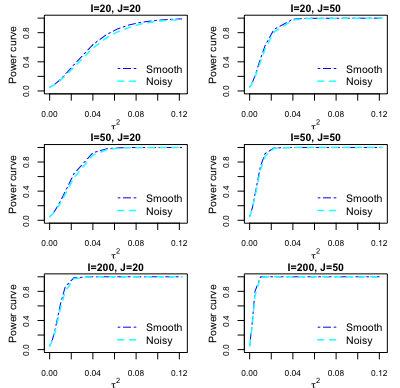
\includegraphics[width=0.9\textwidth]{powercurve.png}
\caption{Power of test ($\tau_k^2=\tau^2$)at the $5\%$ significance level under different model conditions.}
\label{functional power curve}
\end{figure}
In Figure $\ref{functional power curve}$ power curves using both true and noisy $\hat{M}_{I\times J}$ across full combinations of subject number $I$ and visits $J$ are shown. As subject number and visit increase, power of test will be correspondingly increased, and is able to converge to 1 eventually. Under each model condition, test of using true $\hat{M}_{I\times J}$ is more powerful than measurement error considered, i.e. noise added $\hat{M}_{I\times J}$.
\newpage
\subsection{Size Testing To Be Added}
In this section, to compare with our testing procedure, we use the pdIdent model fitting structure in lme approach to fit model under the homoscedasticity assumption, and we would like to show that the size test is too conservative using this method. 

Another method is to fit model under the heteroscedasticity assumption, and then perform multiple test using Bonferroni or benjamini $\&$ Hochberg method.  And we would like to show 
hat the size test is also too conservative using this method. 

\subsection{Power Testing To Be Added}
In the preceding simulation settings, we have shown that our testing procedure by assuming $\tau_k^2=\tau^2$ for all $k$ has good power property when the data is generated following  $\tau_k^2=\tau^2$. In this section, we use heteroscedastic variances $\tau_k^2$ over $k \in \{1,\dots, K\}$ to construct the datasets. Specifically, let $\tau_k^2=\frac{1}{2^{k-1}}\tau^2, k=1,\dots, 3$, and different nonzero $\tau_k^2$s  under the alternative hypothesis are used to generate power curves. 

\begin{figure}[h!]
\centering
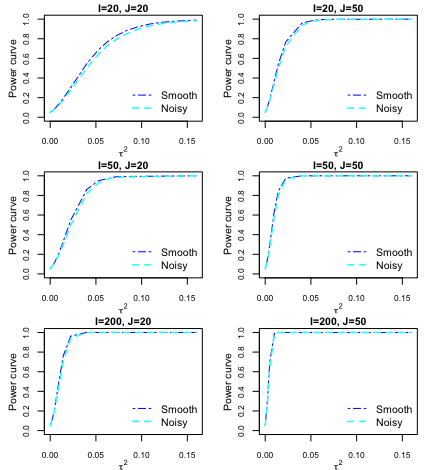
\includegraphics[width=0.9\textwidth]{heter_power_curve.png}
\caption{Power of test ($\tau_k^2=\frac{1}{2^{k-1}}\tau^2$) at the $5\%$ significance level under different model conditions.}
\label{heter functional power curve}
\end{figure}

Figure $\ref{heter functional power curve}$ illustrates the behavior of power when $\tau_k^2$ increases. It shows the similar pattens with data is generated by assuming $\tau_k^2=\tau^2$ for $k \in {1,\dots,3}$ under each of the conditions. That is, power of test will be increased as subject number and visit increase, and power of test will converge to 1. Under each model condition, test of using true $\hat{M}_{I\times J}$ is more powerful than using measurement error added $\hat{M}_{I\times J}$. While under heterogeneous variance, it takes longer for the test of power to increase to 1 compared with using homogeneous variance to construct dataset. 

\subsection{Estimation To Be Added}
Here, in order to evaluate subject-specific derivation $\beta_i(t)$ from the population effect $\beta(t)$ under heteroscedastic variance model, and compare the estimates for population effect $\beta(t)$ from heteroscedastic variance model and no functional random effect model, we consider multiple model conditions.

We generate the response $Y_{ij}$
from model \eqref{eq:lme:approx} with $K=3$, $\delta = 0.5$,
 $\gamma = 2$,
 $\gamma_i \overset{i.i.d.}{\sim} \N(0, 1)$,
 $Z_{ij} \overset{i.i.d.}{\sim} \text{Bernoulli}(0.5)$,
  $\xi_{ijk} \overset{i.i.d.}{\sim} \N(0,\lambda_k)$,
  $\theta = 2$, $\theta_{ik} \overset{i.i.d.}{\sim} \N(0, \tau_i^2)$, $i=1,\dots, K$,
  and  $\epsilon_{ij} \overset{i.i.d.}{\sim} \N(0, 1)$.
  Here, $\lambda_k=0.5^k, k=1,\dots, K$.
 Then the noisy functional data is generated from model \eqref{eq:W}
with $X_{ij}(t) = \sum_{k=1}^K \xi_{ijk} \phi_k(t)$ 
and $e_{ijk}\overset{i.i.d.}{\sim}\N(0,\sigma_W^2)$.
Here, $\phi_1 (t)=\sqrt{2}\mathrm{sin}(2\pi t)$, $\phi_2 (t)=\sqrt{2}\mathrm{cos}(4\pi t)$,$\phi_3 (t)=\sqrt{2}\mathrm{sin}(4\pi t)$, and $\sigma_W^2$ is chosen so 
that the signal to noise ratio in the functional data $r = \sigma_W^{-2}\int_{\tau} r(t,t) \mathrm{d}t$
equals either 0 or 3. Note that $r=0$ corresponds to smooth functional data without noises and 
$r=3$ corresponds to noisy functional data. Finally homogeneous $\tau_i^2$ and heteroscedastic $\tau_i^2$ are considered for variance of interest, to be specific, we take $\tau_1^2=\cdots=\tau_K^2=\tau^2, \tau^2 \in \{0.02, 0.04, 0.08\}$, and $\tau_i^2=\frac{1}{2^{i-1}}\tau^2, i=1,\dots, K, \tau^2 \in \{0.02, 0.04, 0.08\}$ separately. 

A full combination of the number of subject $I$, the number of visits per subject, $J$, the signal to noise ratio $r$ and variance of interest $\tau_i^2 (i=1,\dots,K)$ in the functional data are taken into model conditions consideration. Hence, datasets are constructed under a total of 72 different model conditions: $\big\{(I,J, r, (\tau_i^2, i=1,\dots,K), \tau^2): I\in \{ 20,50,200\}, J\in \{20,50\}, r\in \{0,3\} , (\tau_k^2,  k=1,\dots,K) \in \{ (\tau_1^2=\cdots=\tau_K^2=\tau^2), (\tau_k^2=\frac{1}{2^{k-1}}\tau^2, k=1,\dots, K) \} , \tau^2 \in \{0.02, 0.04, 0.08\} \big\}$.
Under each model condition, 20000 datasets are simulated.

ISE= $\int(\beta(t)-\hat{\beta}(t))^2 \mbox{dt}$ is used to compare estimate performance for population functional effect $\beta(t)$ from heteroscedastic variance model and no functional random effect model. IMSE = $\frac{1}{I} \sum_{i=1}^{I} \int(\beta_i(t)-\hat{\beta}_i(t))^2 \mbox{dt}$ is used for evaluating the subject-specific functional random effect $\beta_i(t)$ estimated by heteroscedastic variance model. Note that ${\beta}(t) = \sum_{k=1}^{K} {\theta}{\phi}_k(t)$, ${\beta}_i(t) = \sum_{k=1}^{K} {\theta}_{ik}{\phi}_k(t), \hat{\beta}(t) = \sum_{k=1}^{K} \hat{\theta}_k\hat{\phi}_k(t)$
and $\hat{\beta}_i(t) = \sum_{k=1}^{K} \hat{\theta}_{ik}\hat{\phi}_k(t)$. MSE=$\frac{1}{I} \sum_{i=1}^{I}\frac{1}{J_i} \sum_{j=1}^{J_i}(y_{ij}-\hat{y}_{ij})^2$ is used to compare predictions from heteroscedastic variance model and no functional random effect model.



\newpage
\section{Real Data Application}
In this section, we conducted a real data application using data from fMRI painful stimulus study we introduced in section 2.  During this painful study, a total number of 20 subjects are asked for the subjective painful rating after corresponding thermal stimuli is given.  Following the thermal stimuli, fMRI machine records the brain activity every 2 seconds from 21 regions of interest (ROI) simultaneously at one's brain for a entire course of 46 seconds. Then the subjective painful rating regarding to the hot/warm stimuli is reported by the individual. For each individual, different amount of visits ranging in [39,48] are taken. We treat the continuously observed brain neural imaging data as a functional covariate, thermal stimuli as a binary categorical covariate,  and subjective rating as scalar response. Then  we applied our proposed functional mixed effect model extending the scalar on function linear
regression for this repeated outcomes.

Test procedures on 21 ROIs show that there are about half which have significant subjective-specific functional random effect at level of 0.05. We picked 3 out of the most significant ROIs (ROI 1, ROI 10, and ROI 19) to visualize difference among $\beta_i(t)$ and compare modeling them with no functional random effect and with heteroscedastic variance on subject-specific brain activity. Figure $\ref{betat}$ shows the

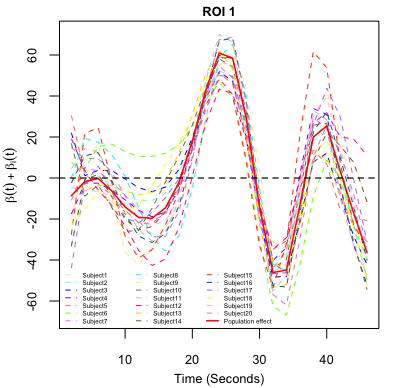
\includegraphics[width=0.48\textwidth]{ROI1_betat.png}
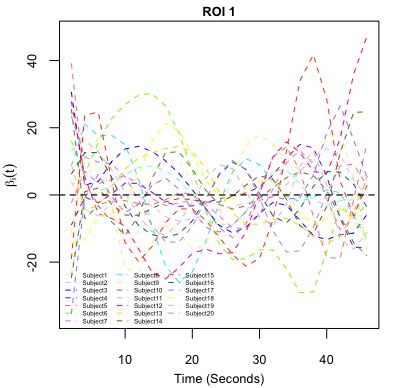
\includegraphics[width=0.48\textwidth]{ROI1_betait.png}

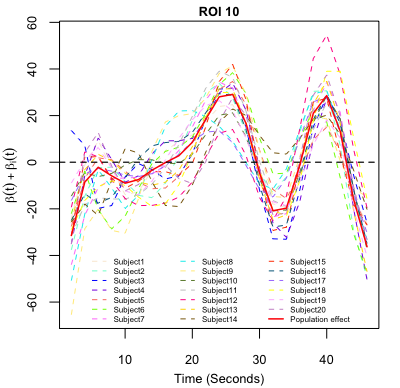
\includegraphics[width=0.48\textwidth]{ROI10_betat.png}
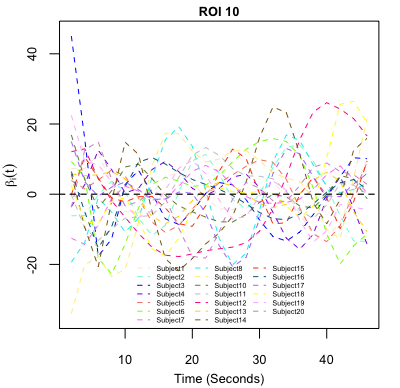
\includegraphics[width=0.48\textwidth]{ROI10_betait.png}

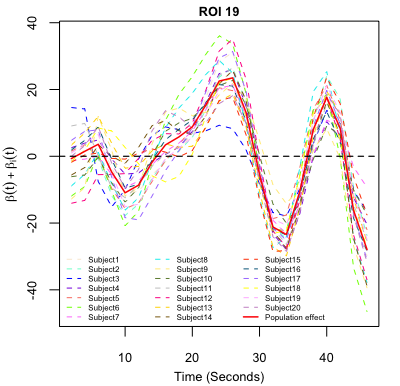
\includegraphics[width=0.48\textwidth]{ROI19_betat.png}
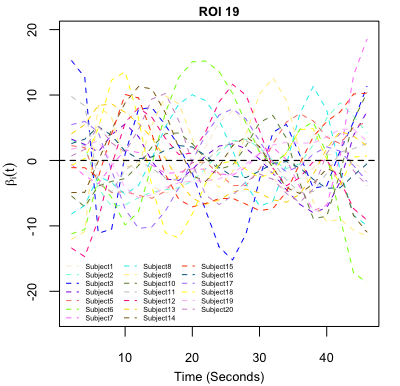
\includegraphics[width=0.48\textwidth]{ROI19_betait.png}

\begin{figure}[h!]
\centering
\caption{Estimates of subject-specific functional mediation effects and subject deviation from the population functional mediation for ROI 1, 10 and 19. In the left panel, the red solid line represents the population functional mediation effect  $\beta(t)$; each of the dashed curve is subject-specific functional mediation effect $ \beta(t) + \beta_i(t)$; In the right panel, each of  the dashed curve is subject-specific deviation $\beta_i(t)$ from the population functional mediation effect $ \beta(t)$. Each subject has the same color across all ROIs.}
\label{betat}
\end{figure}



\begin{table}[!h]
 \caption{RMSE comparison of two models for ROI 1, 10, and 19}   
 \centering
\begin{tabular}{ c | c   c  }\hline\hline
 \multirow{2}{*}{ROI}
  & \multicolumn{2}{c}{RMSE}  \\ \cline{2-3}
  & No random effect  & Heteroscedastic \\
  \cline{1-3}
ROI 1 &  79.236  & 73.67 \\ \cline{1-3}
ROI 10 & 80.649 & 74.64 \\ \cline{1-3}
ROI 19 & 80.39 & 76.67\\
\hline
\hline
 \end{tabular}  
\end{table}
  
%  \begin{table}
%\begin{tabular}{| l | l | l | l | l |}\hline
  %\multirow{1}{*}{Model}  &  & MSE & RMSE & MSE* \\ \cline{1-5}
 %\multirow{2}{*}{Voxel 1}
  %& \multirow{1}{*}{No random effect} & 6278.428 & 79.236 & 6269.934  \\ \cline{2-5}
 % & \multirow{1}{*}{Heterskedastic} & 5428.054 & 73.67 & 5424.417  \\ \cline{2-5}
 % & \multirow{1}{*}{Our model} &  5502.77& 74.181& 5500.03 \\ \cline{2-5}  
 %  \multirow{2}{*}{Voxel 10}
%  & \multirow{1}{*}{No random effect} & 6504.301 & 80.649 & 6496.561  \\ \cline{2-5}
%  & \multirow{1}{*}{Heterskedastic} & 5572.025 & 74.64 & 5570.738  \\ \cline{2-5}
%  & \multirow{1}{*}{Our model} &  5564.165 & 74.59 & 5561.549 \\ \cline{2-5}
%     \multirow{2}{*}{Voxel 19}
%  & \multirow{1}{*}{No random effect} & 6463.045 & 80.39 & 6452.72  \\ \cline{2-5}
%  & \multirow{1}{*}{Heterskedastic} & 5879.517 & 76.67 & 5873.454  \\ \cline{2-5}
%  & \multirow{1}{*}{Our model} &  5833.417& 76.37 & 5826.98 \\ \cline{1-5}
% \end{tabular} 
%  \caption{Model fitting comparison}    
%\end{table}
  
 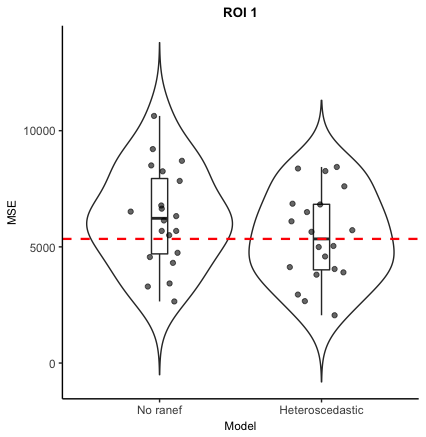
\includegraphics[width=0.45\textwidth]{ROI1_voilin_nohomo.png}
 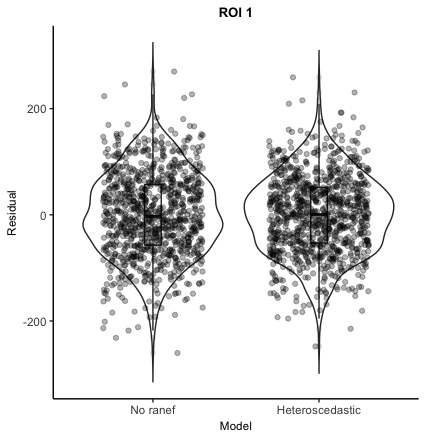
\includegraphics[width=0.45\textwidth]{ROI1_voilin_resi_nohomo.png}
 
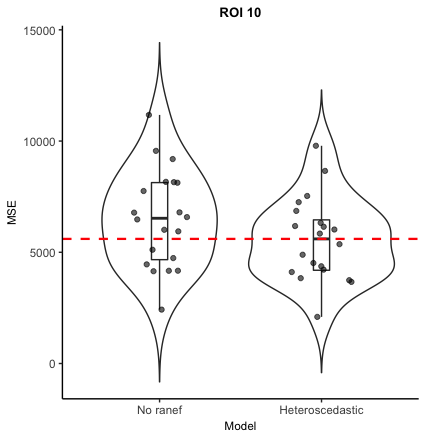
\includegraphics[width=0.45\textwidth]{ROI10_voilin_nohomo.png}
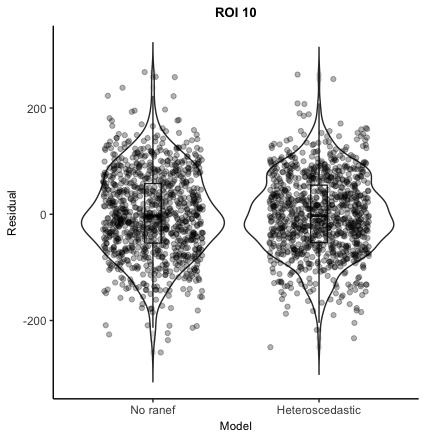
\includegraphics[width=0.45\textwidth]{ROI10_voilin_resi_nohomo.png}

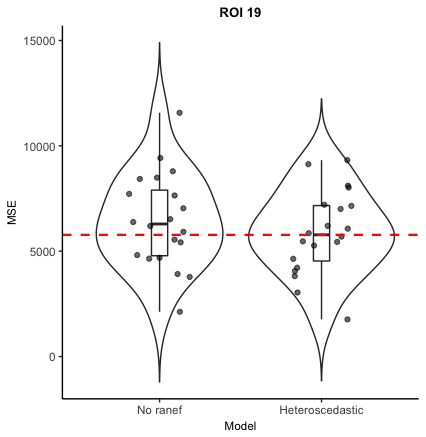
\includegraphics[width=0.45\textwidth]{ROI19_voilin_nohomo.png}
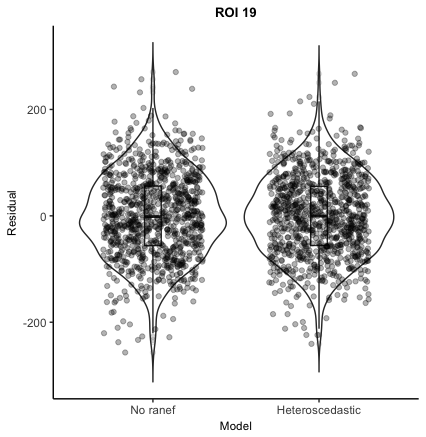
\includegraphics[width=0.45\textwidth]{ROI19_voilin_resi_nohomo.png}

\begin{figure}[h!]
\centering
\caption{Comparison of model fitting between model without subject-level random effect and model with heteroscedastic subject-level random effect for ROI 1, 10 and 19.  Left panel shows the violin plot for MSE of each of 20 subjects in two models; right panel shows the violin plot for 943 residuals in the two models. The red dashed curve represents the median MSE given by Model with heteroscedastic variance}
\label{MSE_voilin}
\end{figure}

%delete figure5
%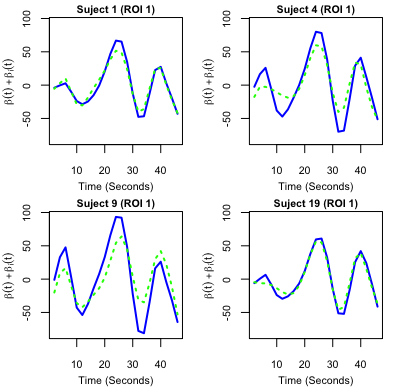
\includegraphics[width=0.45\textwidth]{ROI1_sub4_betat.png}
%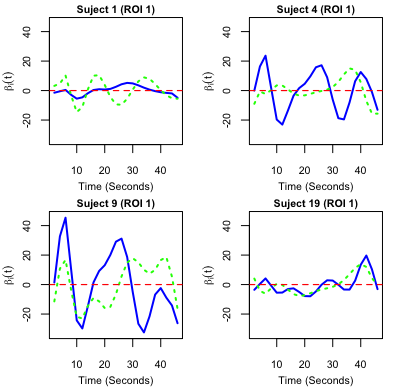
\includegraphics[width=0.45\textwidth]{ROI1_sub4_betait.png}

%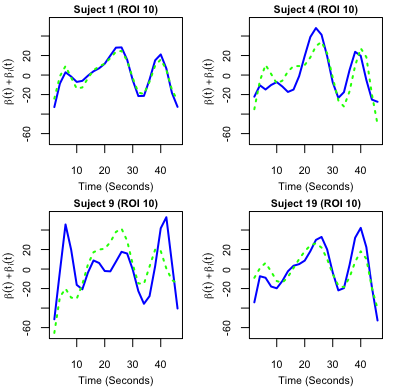
\includegraphics[width=0.45\textwidth]{ROI10_sub4_betat.png}
%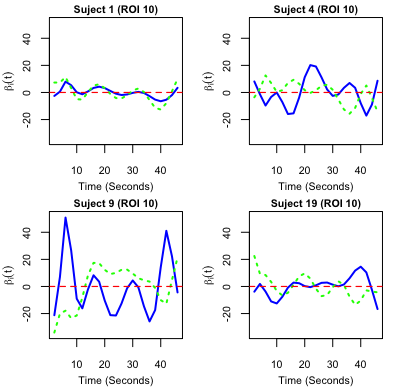
\includegraphics[width=0.45\textwidth]{ROI10_sub4_betait.png}

%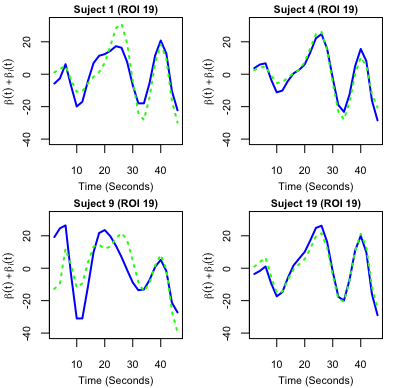
\includegraphics[width=0.45\textwidth]{ROI19_sub4_betat.png}
%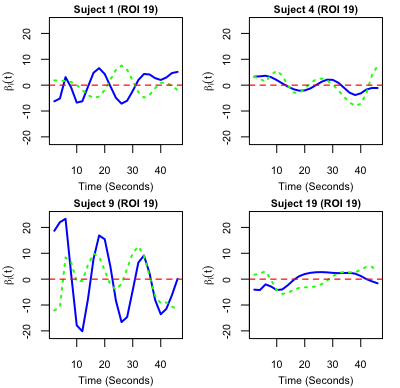
\includegraphics[width=0.45\textwidth]{ROI19_sub4_betait.png}

% \begin{figure}[h!]
%\centering
%\caption{Comparison of estimates of subject-specific functional mediation effects and subject deviation from the population functional mediation of subject1, subject4, subject9, and subject 19 for ROI 1, 10 and 19. In the left panel, the blue solid line represents subject-specific functional mediation effect $ \beta(t) + \beta_i(t)$ given by model with heteroscedastic variance, the green dash line represents $ \beta(t) + \beta_i(t)$ given by model with homogeneous variance; In the right panel, the blue solid line represents subject-specific functional mediation effect  deviation from the population effect $\beta_i(t)$ given by model with heteroscedastic variance, the green dash line represents $\beta_i(t)$ given by model with our method}
%\label{voxel 4sub}
%\end{figure}


\newpage
\bibliography{reference}
\bibliographystyle{plain}
%\section*{Supplementary Material}
\subsection{Simulation Setting}
We generate response $Y_{ij}$ based on the following model

$$
Y_{ij} = \beta_0 + X_{ij} (\beta + \beta_i) + \V{Z}_{ij}\Tra ({b} + \V{b}_i) + \epsilon_{ij}, 
$$

where $\begin{cases} \beta_0 = 0.5 \\ \beta = 2 \\ b = 2 \\ X_{ij} \overset{i.i.d.}{\sim} Bernolli(0.5) \\ \beta_i \overset{i.i.d.}{\sim} Normal(0, 1) \\ \V{Z}_{ij}\Tra = (Z_{ij1}, Z_{ij2}, \cdots, Z_{ijK}) \overset{i.i.d.}{\sim} \mbox{MVN}(\V{0}, \M{I}) \\ Z_{ijk} \overset{i.i.d.}{\sim} Normal(0, 1) \\ \V{b}_i = (b_{1}, b_{2}, \cdots, b_{K})\Tra \overset{i.i.d.}{\sim} \mbox{MVN}(\V{0}, \tau^2\M{I})\\ b_{ik} \overset{i.i.d.}{\sim} Normal(0, \tau^2) \\ \epsilon_{ij} \overset{i.i.d.}{\sim} Normal(0, 1), i\in \{1,\dots,I\}, j\in  \{1,\dots,J\}\\ \end{cases}$.

 Note that $\beta_i$ is a scalar random effect and $\V{b}_i$ is a K-dimensional random effects. Testing $\V{b}_i$, that is, whether $\tau^2=0$ is of our interest. For both size test and power test, we have total sample size $I \in \{20,50,200\}$, and repeated visits $J \in \{20, 50\}$. According to the factorial design, we finally have six model designs $\{(I,J)\}\in \{(20,20),(20,50),(50,20),(50,50),(200,20),(200,50)\}$. Under each of the six model designs, dimension $K$ of the covariate $\V{Z}_{ij}\Tra$ varies in $\{2,4,8\}$. For test of size, we have data generated using $\tau^2=0$, and for test of power, we generate data using multiple different non-zero $\tau^2$ as $\{0.05^2, 0.07^2, 0.1^2, 0.15^2, 0.2^2\}$. Thus for test of size, considering different settings of sample size $I$, repeated visit $J$ and dimension $K$, for all of above $3\times 2\times 3=18$ model settings, we conduct the test $H_0$: $\tau^2= 0$ v.s. $H_a$: $\tau^2 > 0$ through 'exactRLR' based on 20000 times simulation; for test of power, with data generated using multiple different non-zero $\tau^2$, 3 different setting for sample size $I$, 2 different setting for repeated visit $J$ and 3 different settings for dimension $K$, and thus under each of above $18\times 5=90$ model settings, we conduct the test $H_0$: $\tau^2= 0$ v.s. $H_a$: $\tau^2 > 0$ through 'exactRLR' based on 20000 times simulation. For size test, simulated results showing around 5$\%$ type I error rate will be ideal, and for power test, as $\tau^2$ increases, an incremental power curve is expected. We use parallel computing to short the computation time.


\subsection{Simulation Results for Size Test}

\begin{table}[!h]
\caption{Table of size test under 18 model conditions by SVD decomposition transformation}
\centering
\begin{tabular}{c c c c c c c}
\toprule
%\toprule
{Model} & I=20,J=20 & I=20,I=50 & I=50,J=20 & I=50,J=50 &I=200,J=20 & I=200,J=50\\
\midrule
$K=2$ & 0.052 & 0.048 & 0.050 & 0.050 & 0.048 & 0.052 \\ 

$K=4$ & 0.050 & 0.050 & 0.050 & 0.049 & 0.051 & 0.049 \\ 

$K=8$ & 0.050 & 0.052 & 0.048 & 0.049 & 0.051 & 0.049\\ 

\bottomrule
\end{tabular}
\label{tab:sim_results for size test}
\end{table}
 Table 1 provides with the size test results based on 20000 times simulation under full combinations of the simulation design $I \in \{20,50,200\}, J \in \{20,50\}$, $K \in \{2,4,8\}$. As we can see, the test p-values fall in range $[0.048, 0.052]$, which demonstrate that our test procedure can well control type I error around 0.05, and maintain stable performance over change on sample size $I$, visit repeats $J$ and $K$.  
 
\newpage
\subsection{Simulation Results for Power Test}
\begin{figure}[h!]
\centering
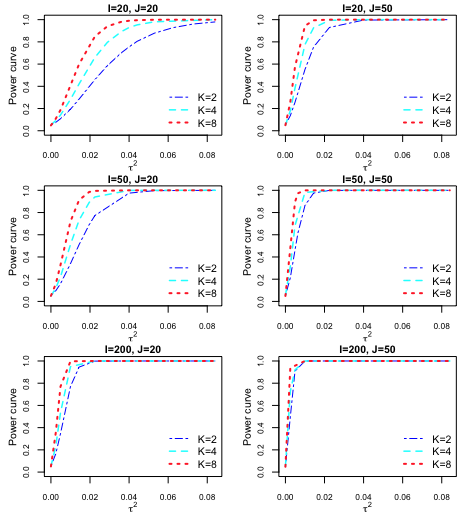
\includegraphics[width=0.9\textwidth]{power_suedo.png}
\caption{Power curve under different sample size $I$, repeated visit $J$, and $K$}
\label{power curve}
\end{figure}

Figure $\ref{power curve}$ illustrates the patten of power as the real variance $\tau^2$ increases from 0 up to $0.21^2$ under 18 different combinations of sample size $I$, repeated visit $J$, and $K$. Under all cases, a monotone increasing power curve with range from approximately 0.05 to 1 is observed. As one would expect, increase on the dimension $K$ of $\V{b}_i$ can lead to increasing test power when sample size $I$ and visit $J$ are fixed. As sample size $I$ increases, power of test will also increase and reach 1 much faster. Increasing visit $J$ can also increase test power. Actually the speed of test power converges to 1 is more sensitive to the affect of visit $J$ than sample size $I$, and thus power will reach 1 faster when $J$ is increased compared with $I$ is increased. For example, comparing the model condition $\{I=20, J=20, K=8\}$ with $\{I=20, J=50, K=8\}$ and $\{I=50, J=20, K=8\}$ respectively, we can see that power reaches over 0.9 at $\tau^2=0.1^2$ and is increased to about 1 at $\tau^2=0.12^2$ when $J$ is changed from 20 to 50 and $I$ stays 20, while power is around 0.7 at $\tau^2=0.1^2$ when $I$ is changed from 20 to 50 and $J$ stay 20. Similar situations can be observed in Figure $\ref{power curve}$.



\end{document}
